\chapter{Experiments}
In this chapter, the quality of the Network and Tracker modules is characterized. First, the available neural networks will be evaluated with a common tracker to obtain the final neural network used for object detection. Second, the tracker implementations will be also characterized using the selected neural network. This will give us the final combination of Network and Tracker module to perform the final experiments. Before these experiments, the configurable parameters will be adjusted to select the best performing values. Finally, the experiments on the final solution are showed.\\
\section{Setup}
The experiments were performed on a laptop PC with \textit{Intel® Core™ i7-4510U CPU @ 2.00GHz x 4} and no GPU acceleration.\\ As commented in section \ref{metrics_tool}, the Object Detection Metrics tool was used for obtaining the following metrics: precision, recall and AP. It is necessary to be mentioned that the tool was modified to provide the TP, FP and GT numbers. The speed measuremenents are obtained directly from the dl-objecttracker in two YML files (for both the Network and the Tracker modules).\\
The dataset selected for evaluating the project is the MOT17Det \textit{train} set (see Table \ref{tab:annex_3}). The results were not evaluated on the \textit{test} set due to the fact that the official web of the challenge does not include in the provided data the annotated ground truth of the test set. To obtain the ground truth from this dataset and adapt it to the metrics tool a little Python script was created following the official reference \cite{milan2016mot16}. However, some modifications were done to allow the compatibility between the metrics tool and the labels of the detections (the neural networks are trained in COCO or PASCAL) (see Table \ref{tab:mot_labels}). Following the official MOT interpretation of ground truth detection files, the final ground truths obtained from the train set only include the \textit{person} class.
\begin{table}[H]
\scriptsize
\begin{center}
\begin{tabular}{|c|l|l|}
\hline
\textbf{ID}                       & \multicolumn{1}{c|}{\textbf{Label in MOT gt}} & \multicolumn{1}{c|}{\textbf{Label in our gt}} \\ \hline
\textbf{1}                        & Pedestrian                                    & Person                                        \\ \hline
\textbf{2}                        & Person on vehicle                             & Car                                           \\ \hline
\textbf{3}                        & Car                                           & Car                                           \\ \hline
\textbf{4}                        & Bicycle                                       & Bicycle                                       \\ \hline
\textbf{5}                        & Motorbike                                     & Motorbike                                     \\ \hline
\textbf{6}                        & Non motorized vehicle                         & Bicycle                                       \\ \hline
\textbf{7}                        & Static person                                 & Person                                        \\ \hline
\textbf{8}                        & Distractor                                    & -                                             \\ \hline
\textbf{9}                        & Occluder                                      & -                                             \\ \hline
\textbf{10}                       & Occluder on the ground                        & -                                             \\ \hline
\textbf{11}                       & Occluder full                                 & -                                             \\ \hline
\multicolumn{1}{|l|}{\textbf{12}} & Reflection                                    & -                                             \\ \hline
\end{tabular}
\end{center}
\caption{Label equivalences with MOT ground truth in our ground truth}
\label{tab:mot_labels}
\end{table}
\section{Neural network}
The correct selection of a neural network model for object detection is crucial in this project as it gives the tracker module the previous detections the tracker needs to track. As commented in section \ref{neural_networks}, the selected neural networks models are:
\begin{itemize}
    \item SSD MobileNetV2, pretrained on COCO (Tensorflow)
    \item Faster R-CNN InceptionV2, pretrained on COCO (Tensorflow)
    \item Mask R-CNN InceptionV2, pretrained on COCO (Tensorflow)
    \item SSD VGG, pretrained on Pascal VOC (Keras)
\end{itemize}
Three sequences from the dataset were selected to evaluate the performance of the models. The reason is that these sequences represent most of the possible difficulties that can appear in multiple object tracking tasks such as occlusions, new targets, fixed camera, big motion from frame to frame, etc. The selected sequences are MOT17-05, MOT17-09 and MOT17-11 (Figure \ref{fig:mot_images})\label{selected_sequences}.\\
\begin{figure}[H]
\begin{center}
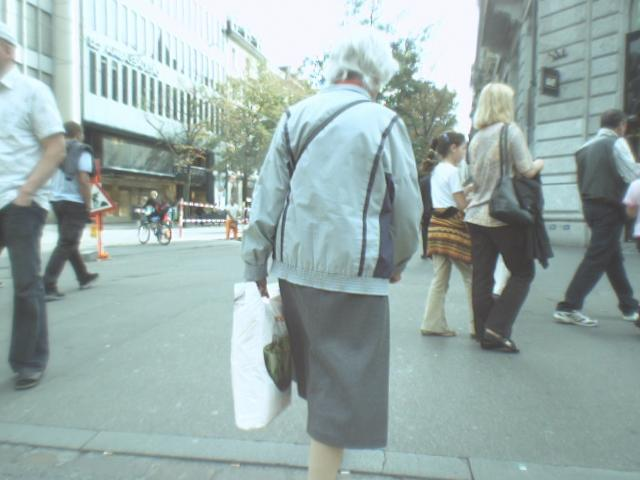
\includegraphics[scale=0.2]{figures/000334.jpg}
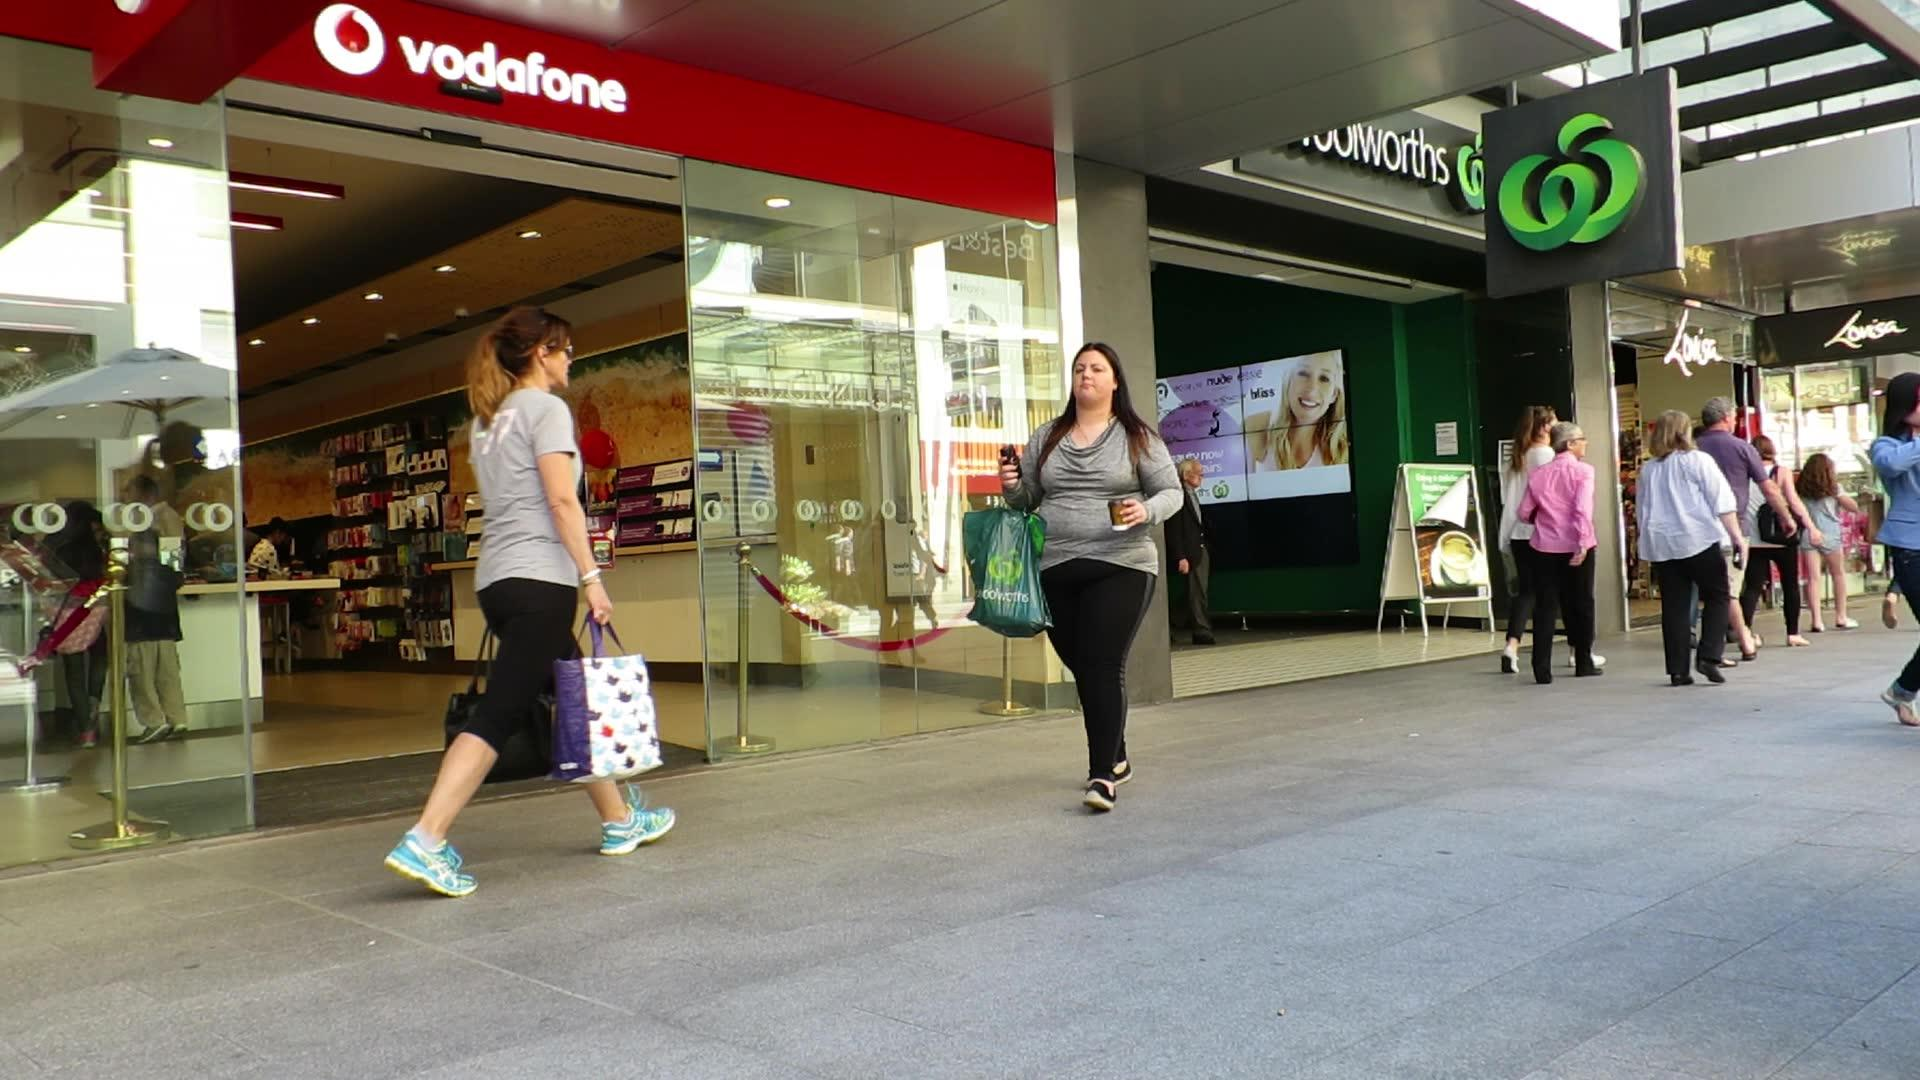
\includegraphics[scale=0.08]{figures/000388.jpg}
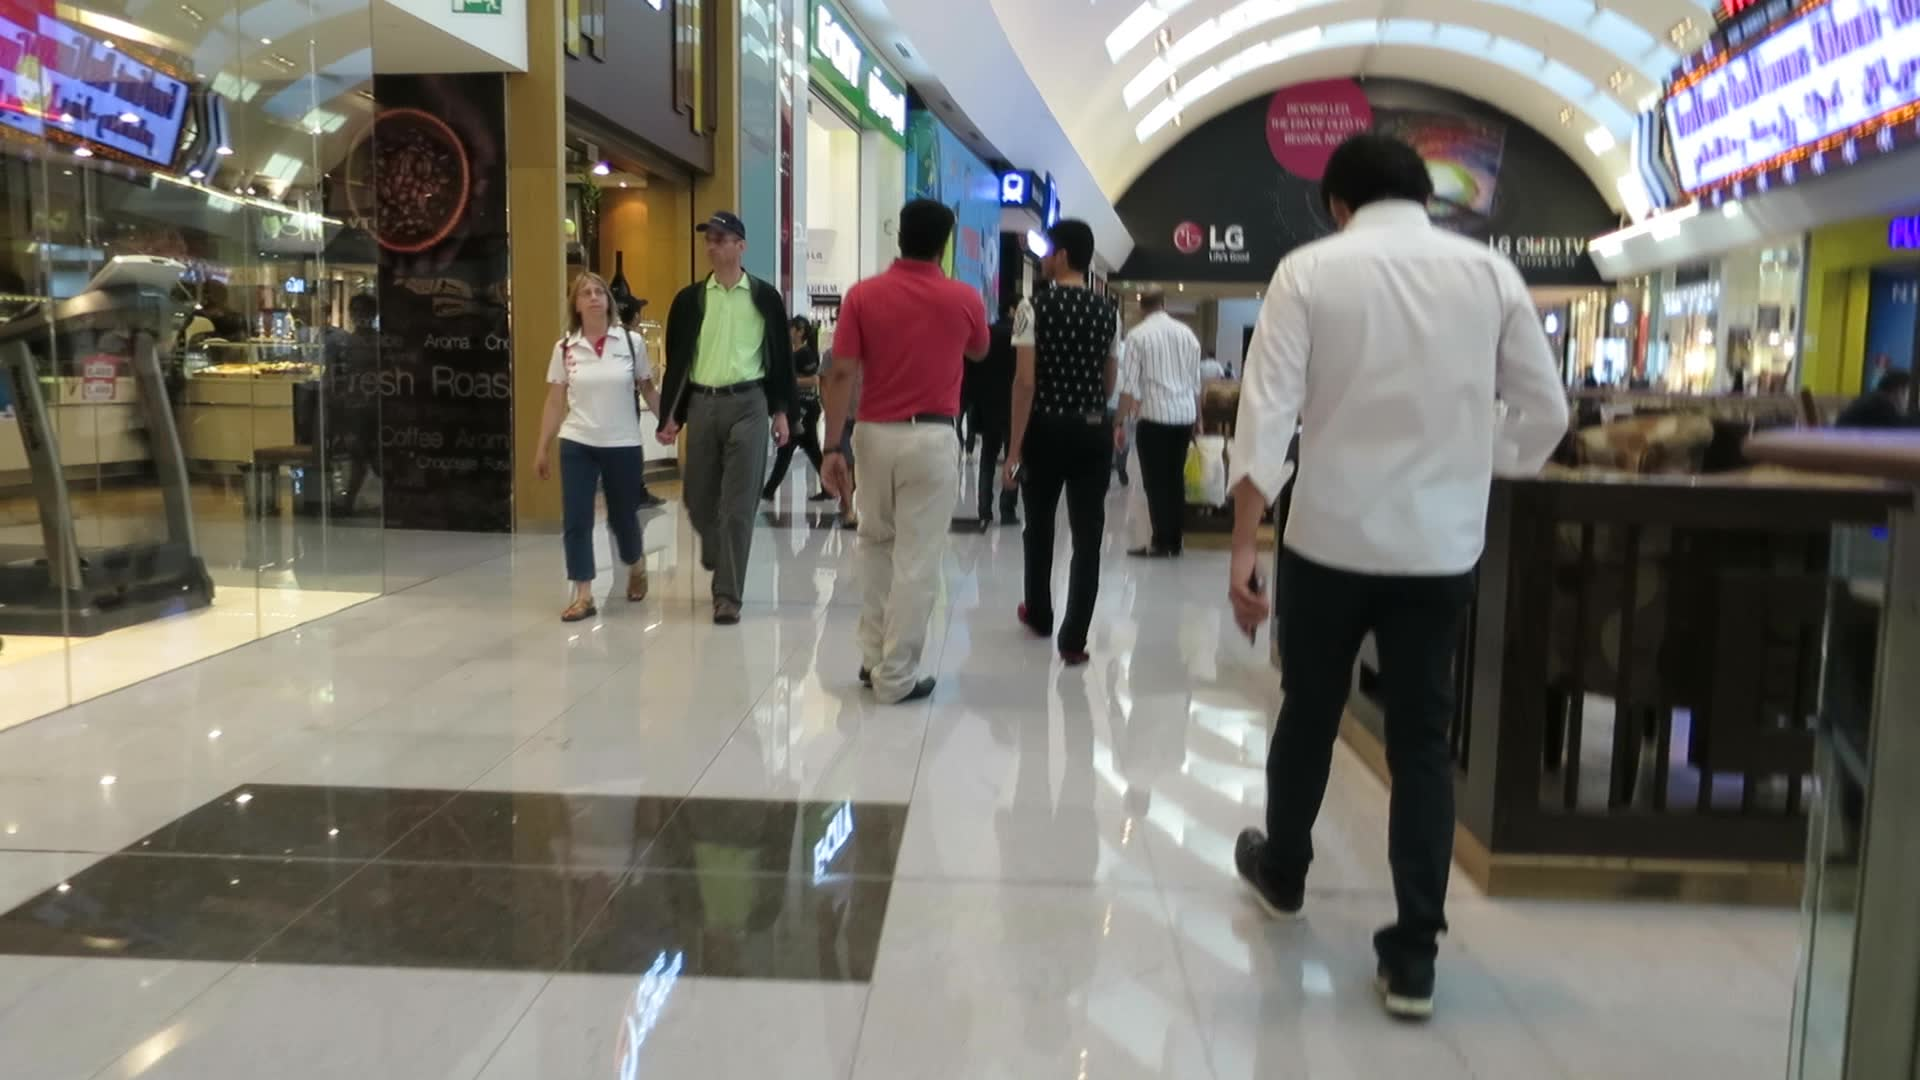
\includegraphics[scale=0.08]{figures/000487.jpg}
\caption{MOT train set samples: left image from MOT17-05, center image from MOT17-09 and right image from MOT17-11}
\label{fig:mot_images}
\end{center}
\end{figure}
The MOSSE tracker was selected as common tracker and the threshold for all neural network detection was fixed to 0,6. This was done to allow a fair comparison between the models.\\
The MOT17-09 sequence has a fixed camera with several pedestrians walking in groups or alone. In this sequence, the tracking can find fast motion difficulties as well as continuous people coming in and out from the scene. To evaluate the performance in the commented sequence, two image inputs sizes were selected due to the Keras SSD-VGG fixed image input size. From the table \ref{tab:net_exp_1}, it can be seen that the maximum AP value is obtained by the Faster R-CNN using 512x512 whereas Mask R-CNN using gets the best AP score for 300x300 images. As expected, the R-CNN detectors obtain the best accuracy. However, this accuracy is not linked with the speed in the object detection. The SSD MobileNetV2 gets the best speed rate in both experiments.\\
\begin{table}[H]
\scriptsize
\begin{center}
\begin{tabular}{|c|c|c|}
\hline
\textbf{}                         & \textbf{AP @ 0,5 (\%)} & \textbf{FPS Net} \\ \hline
\textbf{SSD MobileNetV2}          & 16,06                  & 5,282            \\ \hline
\textbf{Faster R-CNN InceptionV2} & 31,03                  & 1,026            \\ \hline
\textbf{Mask R-CNN InceptionV2}   & 27,89                  & 0,286            \\ \hline
\textbf{SSD VGG 512}              & 23,76                  & 0,339            \\ \hline
\end{tabular}
\end{center}
\caption{Experiments done on MOT17-09 with an image input size of 512x512 in the neural network models}
\label{tab:net_exp_1}
\end{table}
\begin{table}[H]
\scriptsize
\begin{center}
\begin{tabular}{|c|c|c|}
\hline
\textbf{}                         & \textbf{AP @ 0,5 (\%)} & \textbf{FPS Net} \\ \hline
\textbf{SSD MobileNetV2}          & 11,48                  & 8,25             \\ \hline
\textbf{Faster R-CNN InceptionV2} & 24,36                  & 1,067            \\ \hline
\textbf{Mask R-CNN InceptionV2}   & 26,25                  & 0,292            \\ \hline
\textbf{SSD VGG 300}              & 19,08                  & 0,988            \\ \hline
\end{tabular}
\end{center}
\caption{Experiments done on MOT17-09 with an image input size of 320x320 in the neural network models}
\label{tab:net_exp_2}
\end{table}
The influence of the image input size in the speed and the accuracy of the models is clear. In this way, the smaller the input size of the image the faster the detections are obtained. In the opposite way, with a bigger input image the final AP result is better. This trend will be observed in following experiments.\\

The Keras models were discarded for other experiments due to its lack of flexibility because of the fixed input image. In the table \ref{tab:net_exp_3}  it can be observed the different performance from the region-based object detectors with respect to the single-shot object detectors. As it ocurred with smaller image input sizes, the region-based models have a better AP performance almost doubling the AP obtained by the SSD (in the case of Mask R-CNN). For this reason, the SSD MobileNet V2 was eliminated from the neural net selection procedure despite being the faster. 
\begin{table}[H]
\scriptsize
\begin{center}
\begin{tabular}{|c|c|c|}
\hline
\textbf{}                         & \textbf{AP @ 0,5 (\%)} & \textbf{FPS Net} \\ \hline
\textbf{SSD MobileNetV2}          & 17,13                  & 7,372             \\ \hline
\textbf{Faster R-CNN InceptionV2} & 32,00                  & 0,981            \\ \hline
\textbf{Mask R-CNN InceptionV2}   & 34,23                  & 0,272            \\ \hline
\end{tabular}
\end{center}
\caption{Experiments done with an image input size of 800x800}
\label{tab:net_exp_3}
\end{table}
The final experiments will be done on Faster R-CNN and Mask R-CNN in MOT17-09, MOT17-11 and MOT17-05. The last two sequences have a common characteristic which is that the camera is in motion. Thus, the sequences are enumerated in order of increasing degree of motion, starting from MOT-09 to MOT-05.
\begin{table}[H]
\scriptsize
\begin{center}
\begin{tabular}{|c|c|c|c|}
\hline
\textbf{AP @ 0,5 (\%)}            & \textbf{MOT17-09} & \textbf{MOT17-11} & \multicolumn{1}{l|}{\textbf{MOT17-05}} \\ \hline
\textbf{Faster R-CNN InceptionV2} & 35,25             & 26,21             & 19,51                                  \\ \hline
\textbf{Mask R-CNN InceptionV2}   & 31,74             & 26,44             & 12,98                                  \\ \hline
\end{tabular}
\end{center}
\caption{Final net experiments done with an image input size of 1000x1000}
\label{tab:net_exp_4}
\end{table}
From these experiments, it can be seen that the final average precision is similar in the sequence MOT17-11, however, the use of Faster R-CNN model outperforms Mask R-CNN in the other two sequences. These AP scores can be related with the frame rate obtained from each neural network which is about 0,9 FPS for Faster R-CNN and 0,2 FPS for Mask R-CNN. The higher speed can help the tracking procedure to be ``refreshed" more frequently which may lead to better performance on sequences with varying motion between frames as it occurs on the evaluated sequences. In the figure \ref{fig:faster_dets} it can be observed an example of the detections obtained with Faster R-CNN. Generally, the results seem pretty accurated but they include some false positives sucha as the person assigned to a confidence of the 69\%.\\
Given this results, the final neural network chosen to perform the object detection is Faster R-CNN InceptionV2.
\begin{figure}[H]
\begin{center}
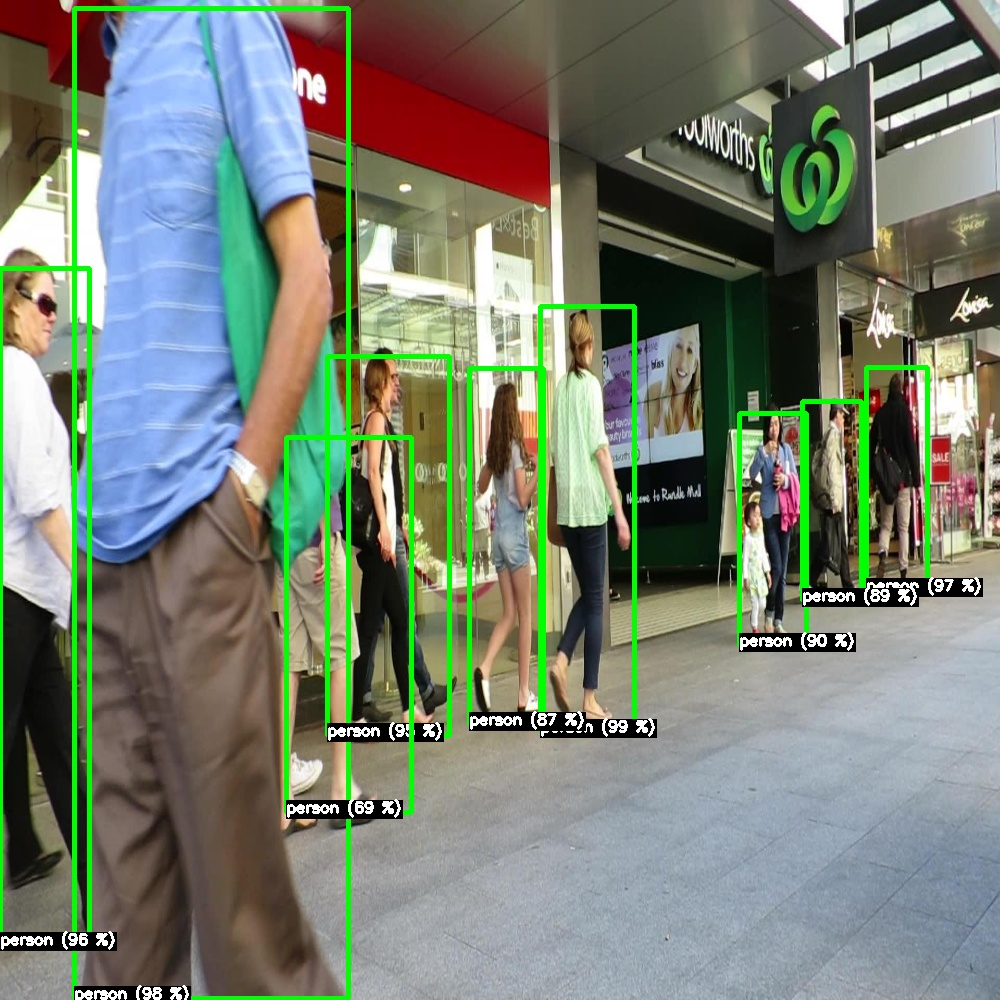
\includegraphics[scale=0.2]{figures/212.jpg}
\caption{Faster R-CNN Inception V2 object detections on MOT17-09}
\label{fig:faster_dets}
\end{center}
\end{figure}
\section{Tracker}
Once the neural network was selected, it is time to evaluate the performance of the second module involved in the core of the multiobject tracking of the application, the tracking algorithm.\\
The following experiments will be done on the same sequences as the Network experiments (section \ref{selected_sequences}). In this case, the default configuration includes Faster R-CNN as neural network with a confidence threshold for detection of 0,6. The confidence of the tracker is being used if no comment is made on it. This confidence is going to be modified to see its influence on the results. The following tracking algorithms are evaluated: KCF, BOOSTING, MIL, TLD, MEDIANFLOW, CSRT, MOSSE and CF-dlib (see section \ref{tracker_algorithms}).\\
\begin{table}[H]
\scriptsize
\begin{center}
\begin{tabular}{|c|c|c|}
\hline
\textbf{}           & \textbf{AP @ 0,5 (\%)} & \textbf{FPS Tracker} \\ \hline
\textbf{KCF}        & \textit{23,07}         & \textit{6,39}        \\ \hline
\textbf{BOOSTING}   & 13,06                  & 4,78                 \\ \hline
\textbf{MIL}        & 15,29                  & 2,21                 \\ \hline
\textbf{TLD}        & 8,38                   & 2,22                 \\ \hline
\textbf{MEDIANFLOW} & \textit{32,13}         & \textit{12,01}       \\ \hline
\textbf{CSRT}       & 11,78                  & 2,78                 \\ \hline
\textbf{MOSSE}      & \textit{34,60}         & \textit{47,07}       \\ \hline
\textbf{CF-dlib}    & \textit{27,99}         & \textit{9,51}        \\ \hline
\end{tabular}
\end{center}
\caption{Tracker experiments done with an image input size of 1000x1000}
\label{tab:tracker_exp_1}
\end{table}
This experiment gives clear results on how its the performance of the trackers in the sequence, thus the KCF, MEDIANFLOW, MOSSE and CF-dlib outperform in a significant way the accuracy of the rest of the trackers (in terms of AP). A good AP seems to be related with a good frame rate in the tracking.
The scheme of evaluating the performance with sequences of increasing difficulty will be followed, the next experiment is going to be evaluated in MOT17-11.

\begin{table}[H]
\scriptsize
\begin{center}
\begin{tabular}{|c|c|c|}
\hline
\textbf{}           & \textbf{AP @ 0,5 (\%)} & \textbf{FPS Tracker} \\ \hline
\textbf{KCF}        & 19,17                  & 4,7                  \\ \hline
\textbf{MEDIANFLOW} & \textit{27,76}         & \textit{12,88}       \\ \hline
\textbf{MOSSE}      & \textit{26,23}         & \textit{33,56}       \\ \hline
\textbf{CF-dlib}    & \textit{25,49}         & \textit{9,95}        \\ \hline
\end{tabular}
\end{center}
\caption{Tracker experiments done with an image input size of 1000x1000}
\label{tab:tracker_exp_2}
\end{table}
The results in this sequence seem to indicate that the KCF tracker is not adecuated for the task. Its results in both AP and speed measurements are below the overall average.
\begin{table}[H]
\scriptsize
\begin{center}
\begin{tabular}{|c|c|c|}
\hline
\textbf{}           & \textbf{AP @ 0,5 (\%)} & \textbf{FPS Tracker} \\ \hline
\textbf{MEDIANFLOW} & \textit{24,01}         & \textit{13,05}       \\ \hline
\textbf{MOSSE}      & 16,15                  & 18,14               \\ \hline
\textbf{CF-dlib}    & 23,97                  & 9,51                 \\ \hline
\end{tabular}
\end{center}
\caption{Tracker experiments done with an image input size of 1000x1000}
\label{tab:tracker_exp_3}
\end{table}
The results from table \ref{tab:tracker_exp_2} lead us to three tracker options that include MEDIANFLOW, MOSSE and CF-dlib. And, after the previous experiment on MOT17-05, MEDIANFLOW gets the overall best performance. It achieves the highest AP score of the three tracker options and the second faster tracking. The faster tracker is MOSSE, following the trend of previous experiments.
\subsection{Confidence in tracking}
In section \ref{tracker_algorithms}, the mechanism of confidence of the tracker was introduced. As commented, the tracker continously checks if the tracking obtained from each tracked object is reliable enough. In this subsection, the importance of this parameter is going to be evaluated. To do so, the performance of the three best tracking algorithms from the previous section is measured when the confidence is taken into account and in the opposite case. The selected sequences are MOT17-05 and MOT17-09 with a frame size of 500x500 and the neural network used is Faster R-CNN InceptionV2.\\
\begin{table}[H]
\scriptsize
\begin{center}
\begin{tabular}{|c|c|c|}
\hline
\textbf{}           & \textbf{AP tracker on @ 0,5 (\%)} & \textbf{AP tracker off @ 0,5 (\%)} \\ \hline
\textbf{MEDIANFLOW} & 36,09                             & 32,35                              \\ \hline
\textbf{MOSSE}      & 18,60                             & 10,33                              \\ \hline
\textbf{CF-dlib}    & 23,74                             & 30,06                              \\ \hline
\end{tabular}
\end{center}
\caption{Confidence influence on tracking performance on MOT17-05}
\label{tab:tracker_exp_4}
\end{table}
\begin{table}[H]
\scriptsize
\begin{center}
\begin{tabular}{|c|c|c|}
\hline
\textbf{}           & \textbf{AP tracker on @ 0,5 (\%)} & \textbf{AP tracker off @ 0,5 (\%)} \\ \hline
\textbf{MEDIANFLOW} & 37,80                             & 36,17                              \\ \hline
\textbf{MOSSE}      & 30,16                             & 21,83                              \\ \hline
\textbf{CF-dlib}    & 28,06                             & 31,60                              \\ \hline
\end{tabular}
\end{center}
\caption{Confidence influence on tracking performance on MOT17-09}
\label{tab:tracker_exp_5}
\end{table}
In the tables \ref{tab:tracker_exp_4} and \ref{tab:tracker_exp_5} the results seem to indicate that the influence of taking into account the confidence parameter with OpenCV trackers is positive. However, it occurs the opposite for the dlib tracking with CF.\\
The MEDIANFLOW tracker is selected to perform the tracking given the performace shown in the previous experiments. In figure \ref{fig:medianflow_images} it can be seen an example of the tracking using the mentioned tracking algorithm.\\
Finally, the image input size was modified to check which size was appropriated to our problem. In table \ref{tab:annex_1}, the image size of 400x400 gets the best balance between speed and accuracy for the tracking task. Given the tracker and the image size, the threshold for the confidence of the detections from the object detection neural networks was evaluated. Using values ranging from 0,3 to 0,7 the experimental selected threshold was 0,5.
\begin{figure}[H]
\begin{center}
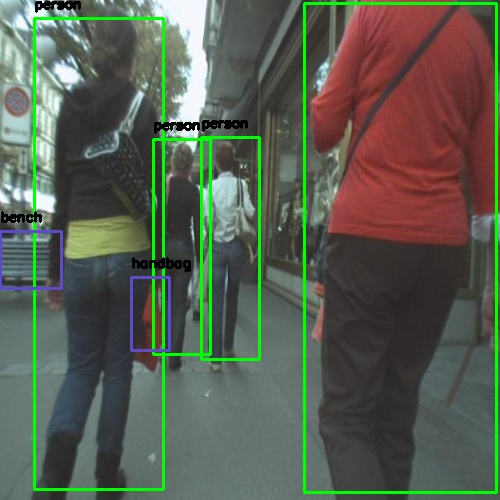
\includegraphics[scale=0.25]{figures/652.jpg}
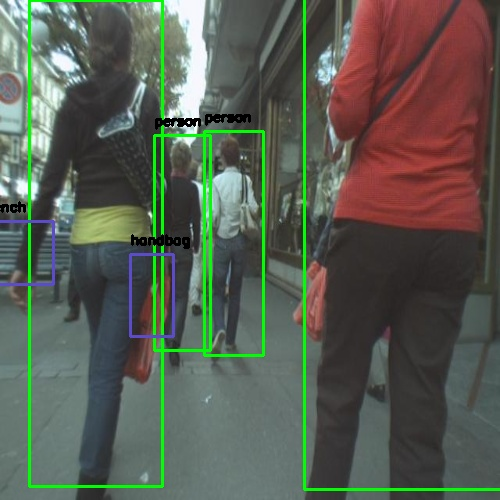
\includegraphics[scale=0.25]{figures/655.jpg}
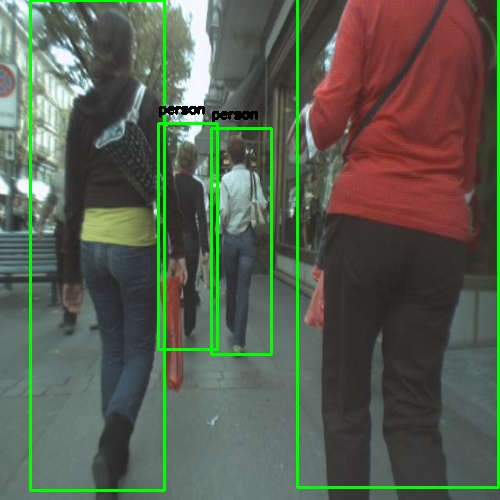
\includegraphics[scale=0.25]{figures/659.jpg}
\caption{Medianflow multiobject tracking on MOT17-05 (selected frames are not sequential)}
\label{fig:medianflow_images}
\end{center}
\end{figure}
\subsection{GOTURN tracking}
The GOTURN (\textit{Generic Object Tracking Using Regression Networks}) is a deep learning based tracking algorithm which learns the motion of the object in an \textit{offline} manner. Many real-time trackers rely on \textit{online} learning that is usually much faster than a deep learning based tracking solution. The authors affirm in the original paper \cite{held2016learning} that they are ``the first neural-network tracker that learns to track generic objects at 100 FPS" (using GPU acceleration, Nvidia GTX 680). However, when using only a CPU the tracker runs at 2,7 FPS according to the authors. This was the main reason to discard this tracker for the project. \textit{Rewrite and comment tests made...} %ToDo: comentar tests con goturn
\section{Final solution}\label{final_sol}
After the experiments run, the project follows the next configuration:
\begin{enumerate}
    \item Neural network: Faster R-CNN InceptionV2, image input size 400x400, confidence threshold 0,5
    \item Tracker: MedianFlow using tracking confidence
\end{enumerate}
Given this configuration, the project is evaluated on the complete train set of MOT17Det to obtain the results of our final solution.
\begin{table}[H]
\begin{center}
\begin{tabular}{|c|c|c|c|}
\hline
\textbf{dl\_objecttracker} & \textbf{AP @ 0,5 (\%)} & \textbf{FPS Net} & \multicolumn{1}{l|}{\textbf{FPS Tracker}} \\ \hline
\textbf{MOT17-02}          & 11,59                  & 0,93             & 31,4                                      \\ \hline
\textbf{MOT17-04}          & 17,25                  & 0,869            & 23,96                                     \\ \hline
\textbf{MOT17-05}          & 36,53                  & 0,98             & 37,28                                     \\ \hline
\textbf{MOT17-09}          & 43,53                  & 0,95             & 35,83                                     \\ \hline
\textbf{MOT17-10}          & 23,26                  & 0,943            & 36,18                                     \\ \hline
\textbf{MOT17-11}          & 35,74                  & 0,96             & 41,56                                     \\ \hline
\textbf{MOT17-13}          & 14,04                  & 0,941            & 42,01                                     \\ \hline
\end{tabular}
\end{center}
\caption{Final results on MOT17Det train set (more detailed results at table \ref{tab:annex_2})}
\label{tab:final}
\end{table}
The best results in terms of average precision occur in the MOT17-09 sequence, followed by MOT17-11 and MOT17-05. This may indicate that the procedure used influences the results giving the better scores in the sequences used to evaluate the performance of the Tracker and Network module. However, from table \ref{tab:annex_2} it can be observed that the three sequences mentioned have in common that they have a smaller number of total ground truth ocurrences. It can be easier for the developed system to get higher results in this type of sequences. Also, from table \ref{tab:annex_3}, the results may indicate that the solution performs best on sequences with lower crowd densities.\\
Refering to velocity of the solution, the object detection in the neural network is returned with a stable frame rate of about 1 FPS. In the case of the tracker, the FPS are above 20 FPS in every sequence.